\section{Loss Normalization and Task Performance}
\label{sec:normalization}

\paragraph{Shared experimental setting.}
We train Qwen3-1.7B with four RL-specialized teachers derived from the same base model, covering mathematics, code, instruction following, and science. Joint training uses 500 updates with 16 fresh responses per domain per update; mathematics-only training uses the same total batch size. Comparisons within each optimizer share initialization, teachers, and prompt schedules. AdamW uses learning rate $2.5\times10^{-7}$, moments $(0.9,0.98)$, and norm-1 clipping. Responses are sampled at temperature 1 with a 4,096-token cap; thinking is disabled throughout.

\paragraph{Evaluation and uncertainty.}
Development scores use MATH-500, LiveCodeBench v6, IFBench, and GPQA Diamond, with 500/1,055/300/198 questions. The first three use greedy decoding; GPQA averages correctness over four sampled responses per question. Evaluation uses a 32,768-token context, and the four-domain mean weights tasks equally. Reported 95\% contrast intervals estimate question-sampling uncertainty through a Gaussian parametric bootstrap calibrated on historical paired-question variances. Table~\ref{tab:main_outcomes} collects the endpoint scores and the separate-test means evaluated in Section~\ref{sec:recipe}.

% Estimated paired intervals: experiments/table1_paired_estimates_20260918/estimate_intervals.py.


% \begin{table}[t]
% \centering\small
% \setlength{\tabcolsep}{3.5pt}
% \caption{\textbf{Task gains and method rankings vary across domains and evaluation sets.} Joint-training scores (\%) after 500 updates; development and separate-test means weight domains equally. Development tasks are MATH-500, LiveCodeBench v6, IFBench, and GPQA Diamond. PG: sampled-token supervision; I16/I64: top-16/top-64 intersection supervision. DR/DT: equal domain weights with response/token averaging; GT: global token averaging. $\Delta$ is the development-mean difference from PG-DR/Adam.}
% \label{tab:main_outcomes}
% \begin{tabular}{@{}lrrrrrrr@{}}
% \toprule
% Configuration & Math & Code & IF & Science & Dev. mean & Test mean & $\Delta$ [95\% interval] \\
% \midrule
% Initial student & 68.80 & 16.41 & 18.33 & 32.20 & 33.94 & 38.60 & $-4.68$ [-6.42, -2.93] \\
% \midrule
% \multicolumn{8}{l}{\textit{Adam}} \\
% PG-DR & 73.20 & 18.27 & 27.00 & 35.94 & 38.61 & 43.55 & Reference \\
% PG-DT & 73.20 & 19.24 & 27.00 & 34.96 & 38.60 & 43.51 & $-0.01$ [-1.45, 1.43] \\
% PG-GT & 76.20 & 17.92 & 27.33 & 32.94 & 38.60 & 44.51 & $-0.01$ [-1.44, 1.42] \\
% I16-DR & 75.40 & 17.75 & 27.00 & 35.98 & 38.90 & 44.56 & $+0.29$ [-1.15, 1.73] \\
% I64-DR & 75.80 & 18.30 & 27.33 & 34.71 & 39.04 & 44.46 & $+0.43$ [-1.01, 1.86] \\
% I64-DT & 74.00 & 18.86 & 28.67 & 35.22 & 39.19 & 43.68 & $+0.58$ [-0.87, 2.02] \\
% I64-GT & 74.20 & 19.80 & 28.67 & 33.41 & 39.02 & 44.97 & $+0.41$ [-1.03, 1.85] \\
% \midrule
% \multicolumn{8}{l}{\textit{SGD}} \\
% PG-DR & 76.40 & 19.53 & 28.33 & 35.59 & 39.96 & 43.48 & $+1.35$ [-0.09, 2.79] \\
% PG-DT & 75.20 & 20.31 & 28.33 & 33.90 & 39.44 & 43.90 & $+0.83$ [-0.61, 2.26] \\
% PG-GT & 75.00 & 19.26 & 25.33 & 34.71 & 38.58 & 42.97 & $-0.04$ [-1.47, 1.40] \\
% \bottomrule
% \end{tabular}
% \par\vspace{2pt}
% \end{table}


\begin{table}[t]
\centering
\small
\setlength{\tabcolsep}{3.5pt}
\caption{\textbf{Task gains and method rankings vary across domains and evaluation sets.}
Joint-training scores (\%) after 500 updates.
Training results are reported as mean $\pm$ standard deviation over three seeds;
the initial student is a single fixed checkpoint.
Development and separate-test means weight domains equally.
Development tasks are MATH-500, LiveCodeBench v6, IFBench, and GPQA Diamond.
PG: sampled-token supervision; I16/I64: top-16/top-64 intersection supervision.
DR/DT: equal domain weights with response/token averaging; GT: global token averaging.}
\label{tab:main_outcomes}
\begin{tabular}{@{}lrrrrr@{}}
\toprule
Configuration & Math & Code & IF & Science & Dev. mean \\
\midrule
Initial student
& 68.80
& 16.40
& 18.33
& 32.20
& 33.94 \\
\midrule
\multicolumn{6}{l}{\textit{Adam}} \\

PG-DR
& $73.20 \pm 0.80$
& $18.26 \pm 0.71$
& $27.00 \pm 1.20$
& $35.94 \pm 1.42$
& $38.60 \pm 0.69$ \\

PG-DT
& $73.20 \pm 0.72$
& $19.24 \pm 0.83$
& $27.00 \pm 1.00$
& $34.93 \pm 1.35$
& $38.60 \pm 0.65$ \\

PG-GT
& $76.20 \pm 0.69$
& $17.91 \pm 0.66$
& $27.33 \pm 1.20$
& $32.91 \pm 1.54$
& $38.59 \pm 0.70$ \\

I16-DR
& $75.40 \pm 0.92$
& $17.73 \pm 0.62$
& $27.00 \pm 1.15$
& $35.98 \pm 1.31$
& $39.03 \pm 0.67$ \\

I64-DR
& $75.80 \pm 0.80$
& $18.29 \pm 0.75$
& $27.33 \pm 1.00$
& $34.68 \pm 1.48$
& $39.03 \pm 0.68$ \\

I64-DT
& $74.00 \pm 1.00$
& $18.86 \pm 0.69$
& $28.67 \pm 1.33$
& $35.19 \pm 1.27$
& $39.18 \pm 0.72$ \\

I64-GT
& $74.20 \pm 0.80$
& $19.78 \pm 0.88$
& $28.67 \pm 1.20$
& $33.38 \pm 1.61$
& $39.01 \pm 0.59$ \\

\midrule
\multicolumn{6}{l}{\textit{SGD}} \\

PG-DR
& $76.40 \pm 0.72$
& $19.53 \pm 0.79$
& $28.33 \pm 1.15$
& $35.56 \pm 1.36$
& $39.96 \pm 0.52$ \\

PG-DT
& $75.20 \pm 0.87$
& $20.28 \pm 0.92$
& $28.33 \pm 1.15$
& $33.88 \pm 1.45$
& $39.42 \pm 0.55$ \\

PG-GT
& $75.00 \pm 1.04$
& $19.24 \pm 0.73$
& $25.33 \pm 1.33$
& $34.72 \pm 1.52$
& $38.58 \pm 0.60$ \\

\bottomrule
\end{tabular}
\par\vspace{2pt}
\end{table}

\subsection{Response length changes the contribution of each domain and response}

Longer responses receive more weight when the loss is averaged over all tokens. In our training batches, mathematics accounts for about three times as many response tokens as instruction following, even though the two domains receive equal numbers of prompts (Figure~\ref{fig:normalization_capability}a). Global token averaging therefore gives mathematics a larger share of the loss. Averaging each domain separately fixes its total contribution; averaging response losses equally also removes the extra weight assigned to long responses.

The remaining effect of length within a domain has a simple form. For response gradients $g_i=\nabla_\theta\ell_i$ and domain means $\bar g_d,\bar T_d$, the token-weighted gradient is
\begin{equation}
\frac{\sum_{i\in\mathcal B_d}T_i g_i}{\sum_{i\in\mathcal B_d}T_i}
=\bar g_d+\frac{\operatorname{Cov}_d(T,g)}{\bar T_d}.
\label{eq:weighting}
\end{equation}
Token averaging retains the length--gradient covariance term; response averaging uses $\bar g_d$. Correcting each domain's global-token contribution by its target weight divided by its observed token share gives domain-token averaging exactly, as in Open-MOPD \citep{gao2026openmopddiagnosingfixingcapability}. This correction preserves within-domain length weighting.

\subsection{Trained Adam moments align updates from different averaging rules}

\paragraph{Different gradients produce closely aligned Adam steps.}
Across six fixed batches at updates 100 and 250 of the sampled-token student, top-64 gradients from equal response weighting and within-domain token weighting have mean cosine 0.68. Each batch contains eight responses per domain and shares student parameters, responses, and teacher scores across averaging rules. Applying those gradients to copies of the same saved Adam state raises their update cosine to 0.96 (Figure~\ref{fig:normalization_capability}b). Comparisons with global token averaging show the same pattern.

\begin{figure}[t]
\centering
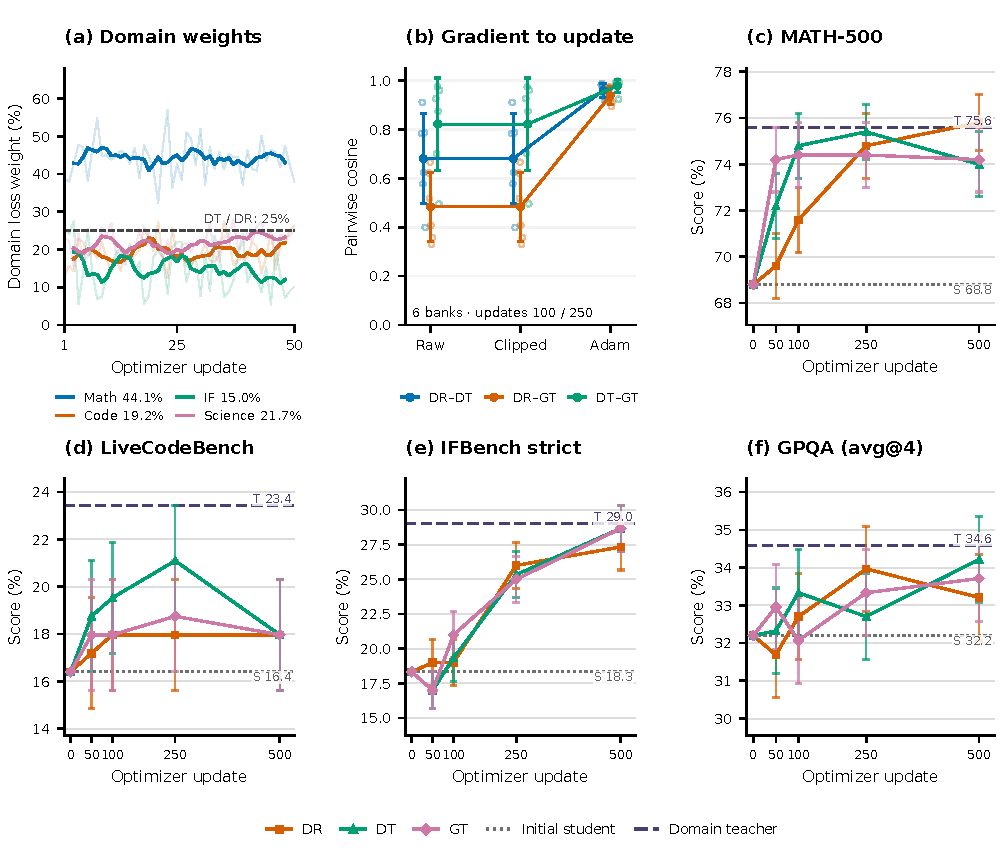
\includegraphics[width=\linewidth]{figures/nine_panel_20260914/section3_normalization.pdf}
\caption{Loss weighting, optimizer mediation, and task capability trajectories.
(a) GT domain loss weights across the first 50 updates: faint lines are individual batches, bold lines are five-batch moving averages, and legend values are arithmetic means over all 50 batches. DT and DR each fix domain weights at 25\%.
(b) Three reduction pairs before clipping, after clipping, and after a shared saved-state Adam update. Small open points are six fixed banks at updates 100/250; lines and error bars show their mean and sample standard deviation.
(c--f) GT/DT/DR scores on MATH-500, LiveCodeBench, IFBench strict, and GPQA (avg@4), with initial-student (S) and domain-teacher (T) references. Points and error bars retain the original means and sample standard deviations, computed from measured seed-42 scores and estimated seed-43/44 scores. The authors report agreement with subsequent three-seed experiments; the retained estimates are not independently verified measurements. Updates use a linear axis. Appendix Figure~\ref{fig:normalization_aggregate_support} gives the four-domain mean and worst-domain change.}
\label{fig:normalization_capability}
\end{figure}


Adam transforms the current gradient through its accumulated first and second moments \citep{kingma2015adam}.

In three SmolLM batches at the exported trained parameters, zero-initialized Adam moments lower the response-versus-token cosine from 0.59--0.90 for raw gradients to 0.41--0.70 for steps. Together, these observations make the optimizer state central to interpreting update alignment.

\paragraph{Clipping preserves gradient direction; optimizer history shapes the step.}
Equal response weighting triggers clipping throughout training, and token weighting triggers it less often (Figure~\ref{fig:normalization_interventions}a). Global norm clipping preserves pairwise gradient cosines. Resetting Adam's moments changes step norms and held-out loss changes, while norm-matched SGD steps separate the averaging rules more strongly (panels b,c). These interventions show how accumulated moments shape the effect of the current gradient.

One-step improvements also vary by domain. We score one held-out response per domain in each batch after BF16 writeback. At update 250, global token averaging changes mean full-vocabulary KL by $-0.027\times10^{-3}$ and instruction-following KL by $+0.272\times10^{-3}$. The aggregate improvement coexists with a domain-level regression.

\begin{figure}[t]
\centering
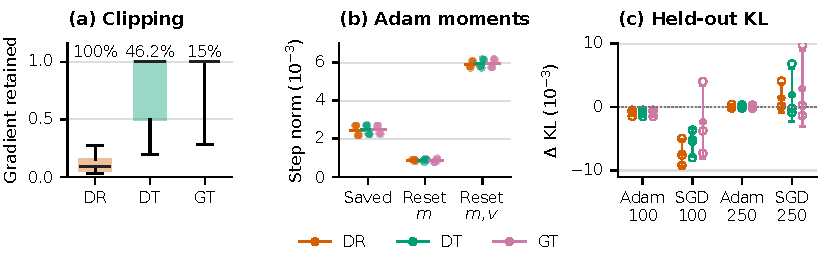
\includegraphics[width=\linewidth]{figures/added_control_figures_20260914/normalization_interventions.pdf}
\caption{Optimizer interventions.
(a) Gradient fraction retained over 500 updates per reduction; labels give clipping rates, boxes the interquartile range, and whiskers the 5th--95th percentiles.
(b) FP32 step norms across six banks; bars show means.
(c) Immediate held-out reverse-KL changes under saved Adam and norm-matched SGD; lower is better. Open points denote banks; filled points and error bars show mean $\pm$ sample SD.}
\label{fig:normalization_interventions}
\end{figure}


\subsection{Final scores are close under Adam, with different task trajectories}

\paragraph{Top-64 supervision yields similar final means across averaging rules.}
The three rules finish within 0.17 percentage points in mean score. Their learning curves and task rankings vary (Figure~\ref{fig:normalization_capability}c--f): all three approach teacher performance on mathematics and instruction following, retain a code gap, and start near the science teacher's score. Domain token averaging exceeds global token averaging by 0.17 mean points, with an estimated 95\% interval of $[-1.27,1.61]$.


\paragraph{The observed score spread is larger with SGD.}
With sampled-token supervision, final mean scores span about 1.4 points under SGD and are nearly tied under Adam. Equal response weighting has the highest observed SGD mean. Its advantage over global token weighting is 1.39 points, with an estimated 95\% interval of $[-0.04,2.82]$. Across the evaluated choices, the initial four-domain mean rises from about 34\% to 39--40\% (Table~\ref{tab:main_outcomes}).

\FloatBarrier
